\chapter{GOTO Hardware Tests and On-Site Commissioning}
\label{chap:commissioning}
\chaptoc{}

% ########################################

\newpage
\section{Introduction}
\label{sec:commissioning_intro}
\begin{colsection}

% ~~~~~~~~~~~~~~~~~~~~

\begin{colsection}

WIP

\end{colsection}

% ~~~~~~~~~~~~~~~~~~~~
\subsection{Something}
\label{sec:something}
\begin{colsection}

WIP

\end{colsection}

% ~~~~~~~~~~~~~~~~~~~~

\end{colsection}

% ########################################

\newpage
\section{Detector characterisation tests}
\label{sec:detectors}
\begin{colsection}

% ~~~~~~~~~~~~~~~~~~~~

\begin{colsection}

It was considered important to carry out a good analysis of the GOTO cameras: firstly to ensure they met the specification given by FLI and secondly to independently test the important characteristics that are unique to each detector.

\end{colsection}

% ~~~~~~~~~~~~~~~~~~~~
\newpage
\subsection{Properties of a CCD}
\label{sec:CCDs}
\begin{colsection}

% ---------
\newpage
\subsubsection{Sources of noise}

There are multiple sources of noise in images taken with CCD cameras \citep{CCDs}:

\begin{itemize}
    \item Shot noise derived from counting photo-electrons from the source object.
    \item Dark current noise, shot noise from thermally generated electrons within the sensor.
    \item Read-out noise from the camera electronics.
    \item Fixed-pattern noise from different sensitivities between pixels.
    \item Bias count, a fixed level of output for each pixel.
\end{itemize}

The shot noise ($\sigma_\text{O}$) comes from photons arriving at the sensor at different times. The photon arrival time is a Poisson distribution, and if the number of electrons counted is $N_O$, for large numbers of photons this tends towards a Gaussian distribution with mean $N_O$ and standard deviation $\sigma_O = \sqrt{N_O}$. When carrying out on-sky astronomical observations the source noise is typically divided into noise from the target object and noise from the background sky, but this is not relevant for the in-lab tests described in this section.

Dark current noise ($\sigma_\text{D}$) is due to electrons produced by thermal excitations, these are indistinguishable from photo-electrons and will increase with exposure time. As this is also a photon counting measurement it also follows a Poisson distribution, so the noise $\sigma_O = \sqrt{D}$ where $D$ is the dark current per pixel. Cooling the cameras will reduce the thermal excitations and therefore reduce the dark current.

Read-out noise ($\sigma_\text{RO}$) depends on the speed data is read out from the CCD.\ The FLI MicroLine cameras read out at a fixed \SI{8}{\mega\hertz}, but other astronomical cameras have variable read-out speeds. As a property of the output electronics the read-out noise is independent of signal or the exposure time used, and therefore it can be represented by a constant value, $\sigma_R = R$, measured in electrons. The MicroLine cameras have two channels with independent readouts, so each will have an independent read-out noise.

Fixed-pattern noise ($\sigma_\text{FP}$) is due to the small differences in size and response between pixels, also known as the \gls{prnu}. Therefore the fixed-pattern noise remains constant between images, but unlike the bias level the fixed-pattern noise increases linearly with the input signal. It can therefore be parametrised as $\sigma_\text{FP} = k_\text{FP}N$ where $k_\text{FP}$ is a dimensionless constant of proportionality describing the fixed-pattern noise as a percentage of the full-well capacity. Scientific CCD cameras typically have very small PRNUs, so $k_\text{FP}$ is usually $<1\%$.

The bias level is a fixed output of counts from each pixel, and is entirely independent of the input signal. It is therefore the easiest noise source to account for, as once a master bias frame has been constructed it can simply be subtracted from each frame. The MicroLine cameras also include an overscan region described previously, which gives an independent measurement of the bias level.

The noises described above (aside from the bias) are all independent Gaussian random variables, and therefore are added in quadrature to get the total noise per pixel

\begin{equation}
    \begin{split}
        \sigma_\text{Total}^2 & = \sigma_\text{O}^2 +
                                \sigma_\text{DC}^2 +
                                \sigma_\text{RO}^2 +
                                \sigma_\text{FP}^2 \\
                              & = N_O + D + R^2 + k_\text{FP}^2{(N_O + D + R)}^2.
    \end{split}
    \label{eq:noise}
\end{equation}

\end{colsection}

% ~~~~~~~~~~~~~~~~~~~~
\newpage
\subsection{The FLI cameras}
\label{sec:FLI}
\begin{colsection}

The KAF-50100 detectors used in the GOTO cameras consists of a $8304 \times 6220$ pixel CCD with $\SI{6}{\micro\metre} \times \SI{6}{\micro\metre}$ square pixels. It has two channels and either two or four outputs. In our case the two-output system is used, and reads out at 8 MHz. The layout of the sensor is shown below in \aref{fig:chip}, adapted from the ON Semi specification sheet.

The primary active region has an area of 8176 $\times$ 6132 pixels. This is the default frame that excludes any of the surrounding test regions.

The full frame of the camera outputs an 8304 $\times$ 6220 array. Surrounding the active area on each edge are 16 active buffer pixels, which are light-sensitive but not considered part of the primary region. Around the edge of the active area is a border of light-shielded dark reference pixels: 29 dark rows at the start, 26 rows at the end and 28 columns on the sides leading each row. These pixels do not respond to light and therefore can be used as a dark reference. At the beginning and end of each row there is also a CTE test column with 4 blank columns either side, as well as a CTE test row at the end of each frame, included for test purposes. Finally there are 10 dummy pixels leading each row, as well as a final pixel used in the readout process. These dummy pixels form an overscan region which can be used to measure and correct for bias signal.

The software allows for a large amount of overscan in either dimension. Overscan pixels in the vertical will appear at the top of the frame, and will appear to have a dark current level picked up as they are transferred down the frame. Horizontal overscan pixels will appear at the end of each channel, i.e.\ running down the centre of the frame, and will only contain values approximating the readout noise.

A sample frame from Camera 2 is shown in \aref{fig:frame}. You can clearly see the extra regions around the frame, with the lower corner expanded in more detail.

\begin{figure}[p]
    \begin{center}
        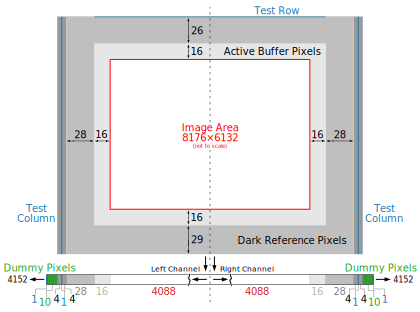
\includegraphics[width=\textwidth]{images/chip}
    \end{center}
    \caption[The layout of the CCD chips in the MicroLine cameras used by GOTO]{
        The layout of the CCD chips in the MicroLine cameras used by GOTO.\@ The central image area is not shown to scale, but the surrounding rows and columns are all in proportion.
        }\label{fig:chip}
\end{figure}

\begin{figure}[p]
    \begin{center}
        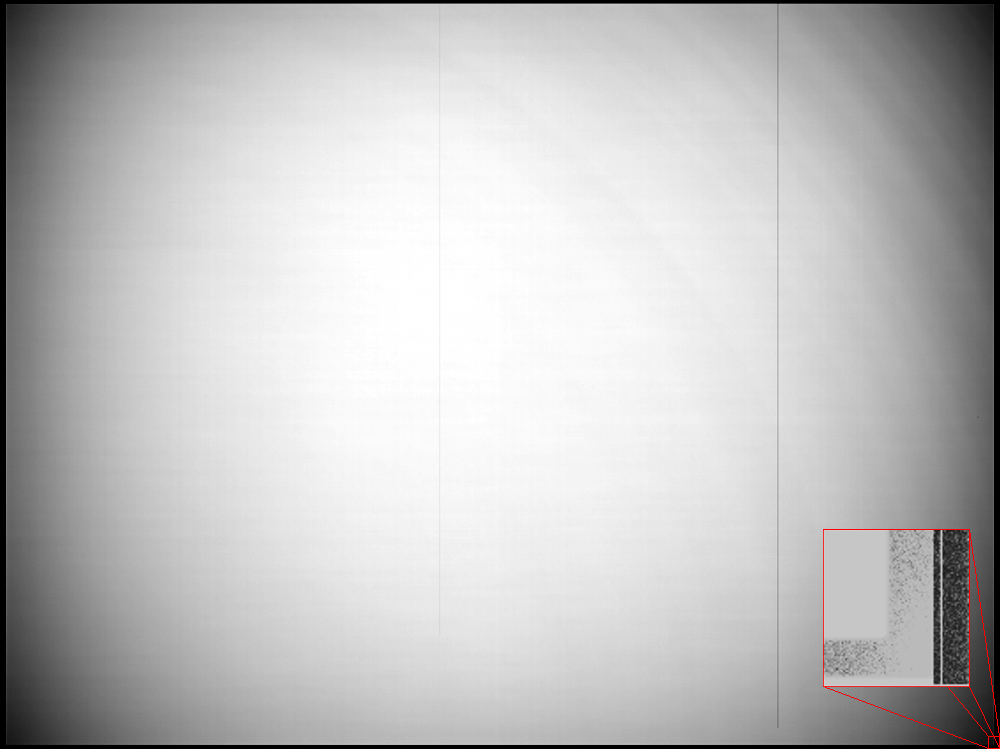
\includegraphics[width=\textwidth]{images/sample.png}
    \end{center}
    \caption[TODO]{
        A sample bright frame from one of the GOTO cameras. The highlighted area in the corner shows some of the features described in \aref{fig:chip}. Also note the two bad columns.
        }\label{fig:frame}
\end{figure}

\clearpage

The first of the FLI cameras to be used on GOTO arrived in Warwick in February 2016, and in March it was moved to Sheffield to carry out a detailed study.
The first camera was bought up to Sheffield on 8th March with a collection of other hardware, it was taken back when the other three were delivered on 10th May. These cameras were returned to Warwick on 8th June.

The results of the analysis were written up as a page on the GOTO wiki for easy access and reference, and are repeated below.

\begin{table}[t]
    \begin{center}
        \begin{tabular}{cccc} %chktex 44
            Name     & Serial number & Set & Tested     \\
            \midrule
            Camera 1 & ML0010316     & 1   & June---??? 2016 \\
            Camera 2 & ML0330316     & 1   & April---June 2016 \\
            Camera 3 & ML0420516     & 1   & June--??? 2016 \\
            Camera 4 & ML0430516     & 1   & June--??? 2016 \\
            \\
            Camera 5 & ML5644917     & 2   & May---June 2018 \\
            Camera 6 & ML6054917     & 2   & May---June 2018 \\
            Camera 7 & ML6094917     & 2   & May---June 2018 \\
            Camera 8 & ML6304917     & 2   & May---June 2018 \\
            \\
            Camera 9 & ML6314917     & --- & --- \\
        \end{tabular}
    \end{center}
    \caption[List of GOTO cameras]{
        A list of the 9 GOTO cameras, with assigned names, serial numbers and when they were tested.
        }\label{tab:cameras}
\end{table}

\end{colsection}

% ~~~~~~~~~~~~~~~~~~~~
\newpage
\subsection{Bias and defects}
\label{sec:bias}
% REMOVE FLI
% Masters are the average of 50 0-s frames
% Then take median of statistics region, in the centre of the frame
% I'm going to have to talk about overscan I fear
\begin{colsection}

\begin{table}[t]
    \begin{center}
        \begin{tabular}{c|rr|rr} %chktex 44
             & \multicolumn{2}{c|}{Sheffield} & \multicolumn{2}{c}{FLI} \\
             & \multicolumn{1}{c}{L} &
               \multicolumn{1}{c|}{R} &
               \multicolumn{1}{c}{L} &
               \multicolumn{1}{c}{R} \\
            \midrule
            Camera 1 &  $971\pm4$ &  $969\pm4$ & $970.6$ &  $965.6$ \\
            Camera 2 &  $989\pm3$ &  $989\pm3$ & $995.7$ &  $988.7$ \\
            Camera 3 & $1004\pm3$ &  $991\pm3$ & $995.6$ &  $989.0$ \\
            Camera 4 &  $974\pm3$ & $1008\pm4$ & $969.7$ & $1000.6$ \\
            Camera 5 &  $994\pm3$ &  $986\pm3$ & $989.8$ &  $978.7$ \\
            Camera 6 &  $984\pm3$ &  $991\pm3$ & $968.1$ &  $976.8$ \\
            Camera 7 &  $992\pm3$ &  $981\pm3$ & $984.2$ &  $975.6$ \\
            Camera 8 & $1008\pm3$ & $1012\pm3$ & $995.5$ &  $996.9$ \\
        \end{tabular}
    \end{center}
    \caption[TODO]{
        Bias levels (in ADU) measured in Sheffield and from the FLI test sheets.
        }\label{tab:bias}
\end{table}

\begin{table}[t]
    \begin{center}
        \begin{tabular}{c|rr|rr|rr} %chktex 44
            &
            \multicolumn{2}{c|}{1$\times$1 binning} &
            \multicolumn{2}{c|}{2$\times$2 binning} &
            \multicolumn{2}{c}{3$\times$3 binning}
            \\
             &
            \multicolumn{1}{c}{L} &
            \multicolumn{1}{c|}{R} &
            \multicolumn{1}{c}{L} &
            \multicolumn{1}{c|}{R} &
            \multicolumn{1}{c}{L} &
            \multicolumn{1}{c}{R}
            \\
            \midrule
            Camera 1 &  $971\pm4$ &  $969\pm4$ & $1036\pm5$ & $1022\pm5$ & $1145\pm7$ & $1127\pm6$\\
            Camera 2 &  $989\pm3$ &  $989\pm3$ & $1045\pm4$ & $1038\pm4$ & $1152\pm6$ & $1143\pm6$\\
            Camera 3 & $1004\pm3$ &  $991\pm3$ & $1060\pm4$ & $1054\pm4$ & $1153\pm5$ & $1149\pm5$\\
            Camera 4 &  $974\pm3$ & $1008\pm4$ & $1031\pm4$ & $1063\pm4$ & $1122\pm5$ & $1155\pm6$\\
        \end{tabular}
    \end{center}
    \caption[TODO]{
        Bias levels (in ADU) for different binning factors.
        }\label{tab:bias_bins}
\end{table}

For a standard full-frame image there are two methods to correct for bias: using the overscan regions and using a master bias.

The two 10-pixel wide dummy regions on either side of the image as shown in \aref{fig:chip} can be subtracted from the frame (independently for each channel) to correct for much of the bias level. These levels change for each image, but typical values for each camera and channel are given in \aref{tab:bias} --- they are usually between 960 and 990 counts.

For each camera 50 dark, zero-exposure full-frame images were taken, overscan subtracted and stacked in order to construct a master bias frame. This can be used to correct for any structure in the bias level. The most obvious structure is a difference in bias levels between the two channels in each camera. The average remaining field bias values are also listed in \aref{tab:bias}.

\begin{table}[t]
    \begin{center}
        \begin{tabular}{cc|lll} %chktex 44
            Camera   & Serial    & \multicolumn{3}{c}{Dark Columns} \\
            \midrule
            Camera 1 & ML0010316 & 1 dead column:  & x=7678, starting at y=4312 & (30\%) \\
            Camera 2 & ML0330316 & 2 dead columns: & x=3583, starting at y=909  & (85\%) \\
                     &           &                 & x=6386, starting at y=127  & (98\%) \\
            Camera 3 & ML0420516 & 2 dead columns: & x=1800, starting at y=1151 & (81\%) \\
                     &           &                 & x=5140, starting at y=4986 & (19\%) \\
            Camera 4 & ML0430516 & 1 dead column:  & x=5333, starting at y=2561 & (58\%) \\
        \end{tabular}
    \end{center}
    \caption[TODO]{
        Locations of dead columns caused by stuck pixels. The percentages denote the amount of the column that is unusable.
    }\label{tab:frame}
\end{table}

For each camera a defect mask was constructed using the ratio of two flat images of different exposures, and then detecting pixels outside of a given sigma limit. Each camera was found to have at least one stuck pixel, which produced a dead column travelling up the frame. In \aref{fig:frame} these are visible as two dark columns. The exact positions and details for every camera are shown in \aref{tab:frame}.

The ONSemi chip specifications gives an allowed limit of less than 20 column defects per device, and none of the GOTO detectors had more than two.

\end{colsection}

% ~~~~~~~~~~~~~~~~~~~~
\newpage
\subsection{Photon transfer curves}
\label{sec:ptc}
% https://harvestimaging.com/blog/?p=1034
% https://www.couriertronics.com/docs/notes/cameras_application_notes/Photon_Transfer_Curve_Derivation.pdf
% http://slittlefair.staff.shef.ac.uk/teaching/phy217/lectures/instruments/L14/index.html
% https://www-spiedigitallibrary-org.sheffield.idm.oclc.org/ebooks/PM/Scientific-Charge-Coupled-Devices/eISBN-9780819480392/10.1117/3.374903
\begin{colsection}

The \gls{ptc} is a method to determine the gain, read-out and fixed-pattern noise for a CCD camera \citep{CCDs, PTC}. To construct a photon transfer curve a series of bright exposures of a flat light source were taken with varying exposure times. For these images the dark current noise is negligible, so once the images has the bias level subtracted the total number of electrons in each pixel, $N_\text{Total}$, will include a number of  photo-electrons from the source $N_O$ plus extra electrons from the readout electronics $R$:

\begin{equation}
    N_\text{Total} = N_O + R.
    \label{eq:total_count}
\end{equation}

The noise per pixel, excluding dark current, is given by \aref{eq:noise} as

\begin{equation}
    \begin{split}
        \sigma_\text{Total}^2 & = N_O + R^2 + k_\text{FP}^2{(N_O + R)}^2 \\
                              & = N_\text{Total} - R + R^2 + k_\text{FP}^2N_\text{Total}^2.
    \end{split}
    \label{eq:ptc_noise1}
\end{equation}

The counts and total noise here are all in electrons (\elec), however the output of the camera analog-to-digital converter is a digital signal, $S$, measured in \gls{adu}. This signal is linearly related to the actual number of electrons detected $N$ through the gain $g$, in \elec/ADU, as

\begin{equation}
    N = g S.
    \label{eq:gain}
\end{equation}

The gain is an important parameter of a CCD detector, and can be set to best utilise the dynamic range of the detector. The KAF-50100 detectors have a specification full well capacity of 40,300 electrons before they saturate, and the cameras have a 16-bit readout (meaning the signal from each pixel can vary from 0 to 65535 ($2^{16}$) ADU). Therefore if the gain was set to $1$ \elec/ADU a saturated pixel would produce a signal of 40300 ADU, which is only using two-thirds of the dynamic range. The ideal gain to utilise the full well capacity for these cameras would therefore be $0.62$ \elec/ADU.\@ However, a high gain introduces a quantisation error due to the random electrons produced by the read-out noise. Setting the gain therefore is a balance between these two effects.

Since \aref{eq:gain} shows the signal $S$ is directly proportional to the number of electrons $N$, their errors are also directly proportional with the same constant. Therefore the noise in the signal, $\sigma_S$, is related to the noise in the electron count as

\begin{equation}
    \sigma_N = g \sigma_S.
    \label{eq:noise_gain}
\end{equation}

Converting the total electron count and noise in \aref{eq:ptc_noise1} into ADU results in

\begin{equation}
    g^2\sigma_S^2 = gS - R + R^2 + k_\text{FP}^2 g^2 S^2,
    \label{eq:ptc_noise2}
\end{equation}

and rearranging this gives the final photon transfer curve equation

\begin{equation}
    \sigma_S^2 = \frac{R^2 - R}{g^2} + \frac{1}{g}S + k_\text{FP}^2 S^2.
    \label{eq:ptc}
\end{equation}

This is a quadratic equation in $S$ which relates the measured total signal $S$ to the variance in the signal $\sigma_S^2$, where $S$ and $\sigma_S$ are in ADU, read-out noise $R$ is still in \elec, gain $g$ is in \elec/ADU and the fixed-pattern noise parameter $k_\text{FP}$ is dimensionless.

A photon transfer curve is a log-log plot of a signal value against the noise in the signal, here represented by $S$ and standard deviation $\sigma_S$ (the square root of the variance). By fitting \aref{eq:ptc} to this plot values for the gain, read-out noise and fixed-pattern noise can be determined. The key features of a photon transfer curve are common for all CCDs, and are shown in cartoon form in \aref{fig:ptc_cartoon}.

\newpage

\begin{figure}[t]
    \begin{center}
        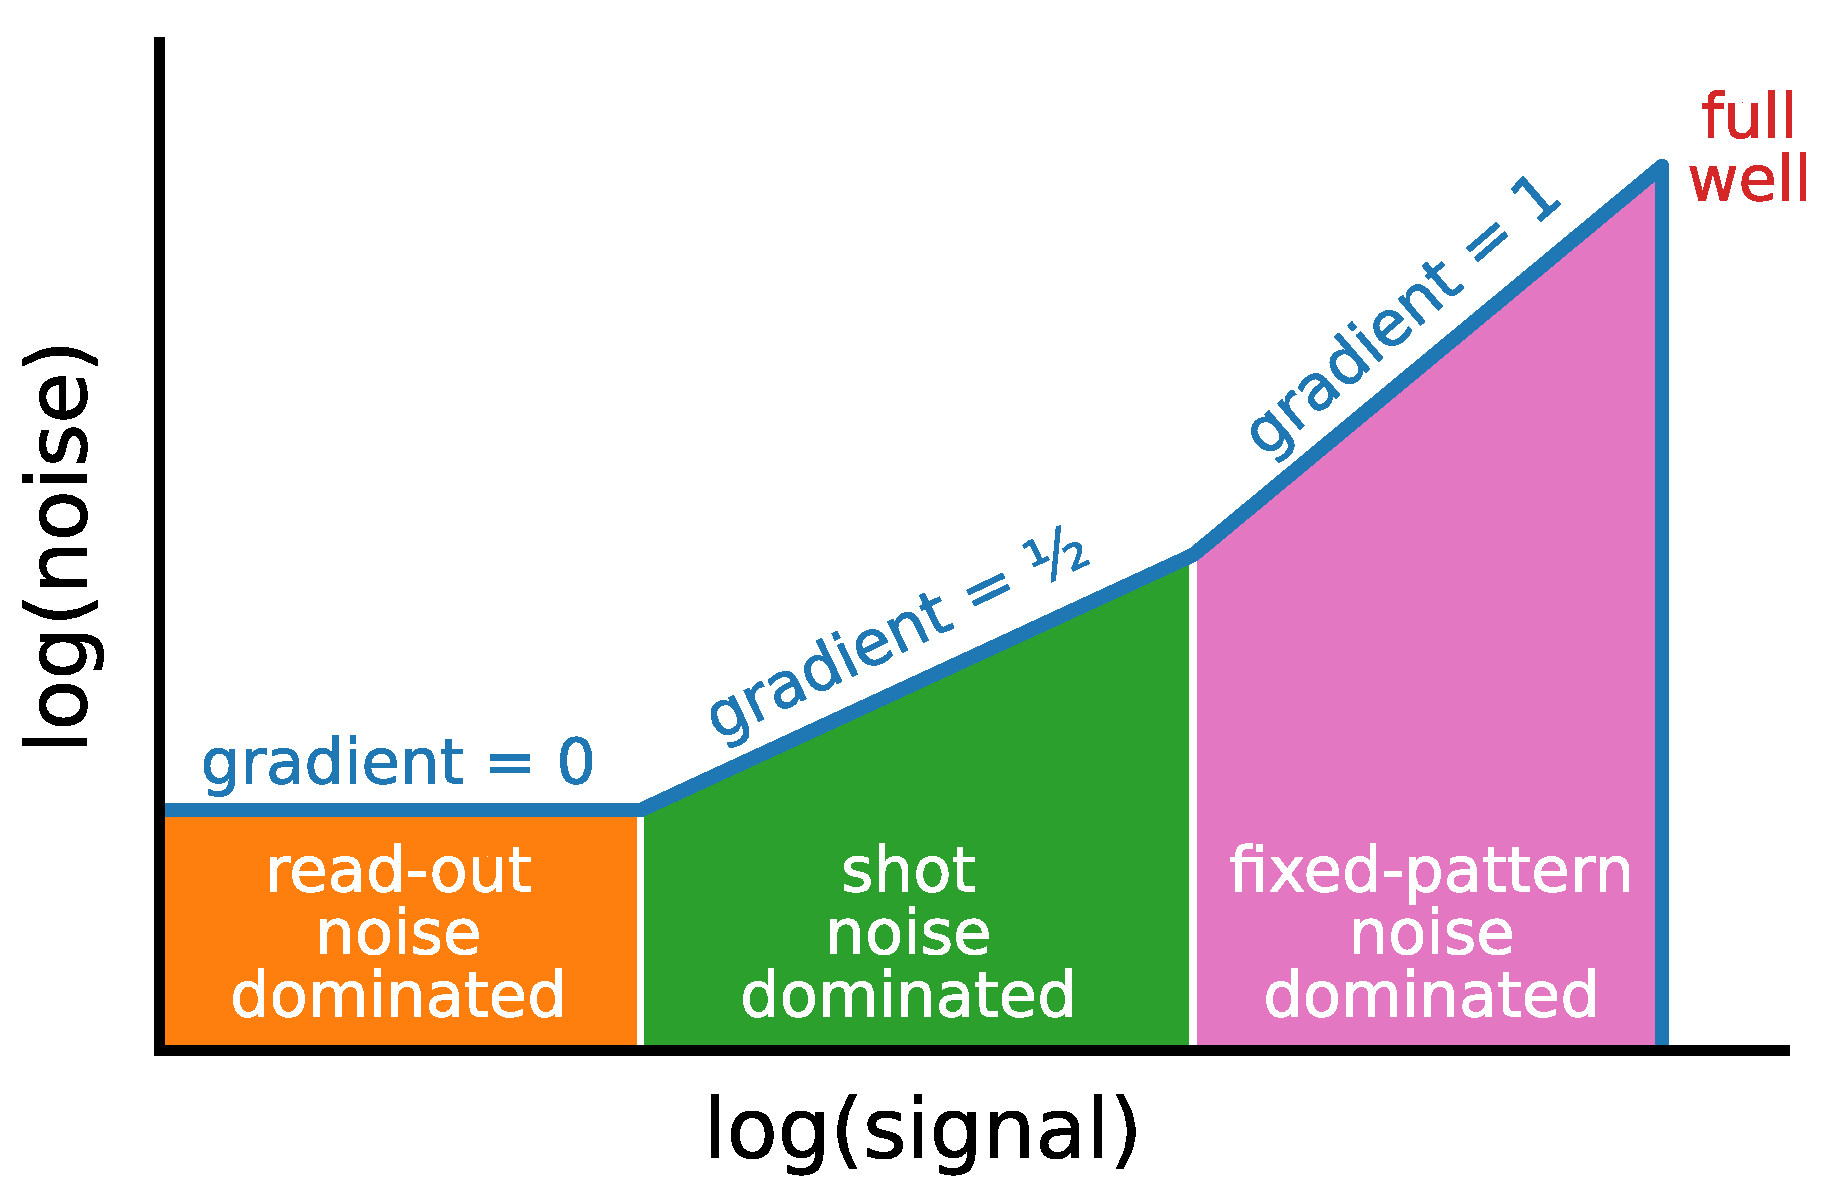
\includegraphics[width=0.65\textwidth]{images/ptc.pdf}
    \end{center}
    \caption[Key features of the photon transfer curve]{
        The key features of a photon transfer curve, adapted from Figure 2.2 of \citet{CCDs}.
        }\label{fig:ptc_cartoon}
\end{figure}

There are three visible noise regimes in the photon transfer curve. The first is when the signal is zero. For small $S$ in \aref{eq:ptc} the noise is constant, and as there is no signal the overall noise is limited by the detector noise. This will include both the read-out noise and the dark current, but as these are very short exposure times (less than 1 second) the dark current is completely negligible and the read-out noise dominates. At higher signals the noise is dominated by the shot noise. As this is proportional to the square root of the signal this region has a gradient of 1/2 when plotted on the log-log axis, and when $\sigma_S$ is zero the signal will equal the gain (i.e.\ the value of the gain is where the linear fit crosses the x-axis). As the signal increases further the fixed-pattern noise begins to dominate over the shot noise, as it is proportional to the signal this produces a gradient of 1 in the \gls{ptc}. Finally the pixel will reach its full well value and saturate, so the noise drops to zero.

As it is impossible to know the exact number of incoming photons on each pixel, it is not possible to determine the signal and noise values for a given pixel. Instead the PTC is constructed by selecting a region of pixels and plotting the mean signal value against the standard deviation. Repeated for several regions across the image this gives a reasonable approximation of the average noise in each pixel.

\newpage

\begin{table}[t]
    \begin{center}
        \begin{tabular}{l|cc|cc|cc} %chktex 44
             &
            \multicolumn{2}{c|}{Gain} &
            \multicolumn{2}{c|}{RO noise} &
            \multicolumn{2}{c}{FP noise} \\
            &
            \multicolumn{2}{c|}{(\elec/ADU)} &
            \multicolumn{2}{c|}{(\elec)} &
            \multicolumn{2}{c}{(\%)} \\
             & L & R & L & R & L & R \\
            \midrule
            Camera 1 & 0.53 & 0.53 & 12.9 & 12.6 & 0.46 & 0.45 \\
            Camera 2 & 0.53 & 0.53 & 12.4 & 12.2 & 0.44 & 0.46 \\
            Camera 3 & 0.57 & 0.57 & 13.1 & 12.3 & 0.45 & 0.42 \\
            Camera 4 & 0.57 & 0.58 & 14.0 & 14.5 & 0.41 & 0.43 \\
            Camera 5 & 0.62 & 0.63 & 12.8 & 13.3 & 0.40 & 0.40 \\
            Camera 6 & 0.63 & 0.62 & 12.4 & 13.1 & 0.40 & 0.40 \\
            Camera 7 & 0.62 & 0.62 & 13.6 & 13.1 & 0.41 & 0.39 \\
            Camera 8 & 0.62 & 0.62 & 14.8 & 12.8 & 0.41 & 0.39 \\
        \end{tabular}
    \end{center}
    \caption[TODO]{
        Results of fitting photon transfer curves for each of the eight cameras.
        }\label{tab:ptc}
\end{table}

\glspl{ptc} were constructed for all eight cameras, by taking flat images of varying exposure times. Twelve 50$\times$50 pixel regions were selected across the field, and the mean and standard deviation of the pixel values were plotted to form the \gls{ptc}. These are shown in \aref{fig:ptcs}. The curves were fitted to \aref{eq:ptc}, and the resulting values for the gain ($g$), read-out noise ($R$) and fixed-pattern noise ($k_\text{FP}$) are given in \aref{tab:ptc}.

As expected, the gain values are all around 0.6 \elec/ADU, and would have been set as such to maximise the dynamic range. There is a clear difference in gain levels between the first set of cameras (1--4) and the second set (5--8), which is most likely due to changes made by FLI over the two years between their manufacture. The read-out noise values match the FLI specifications which advertises a typical system noise of 12 \elec{} when reading out at \SI{8}{\mega\hertz}. The two channels on each camera are independent and therefore there is no correlation in read-out noise, unlike the gain which is always approximately the same in each amplifier. Finally the fixed-pattern noise is always below 0.5\% of the signal as expected. The fraction notably decreases from $\sim$0.45\% to $\sim$0.40\%; if this is related to improved chip manufacturing this might explain the reason FLI were able to set the gain higher for the later cameras. However, this test only includes a small sample of the 50 million pixels on each chip, and so might not be a perfect measure of the overall photo response non-uniformity.

\begin{figure}[p]
    \begin{center}
        \begin{minipage}[t]{0.49\textwidth}\vspace{10pt}
            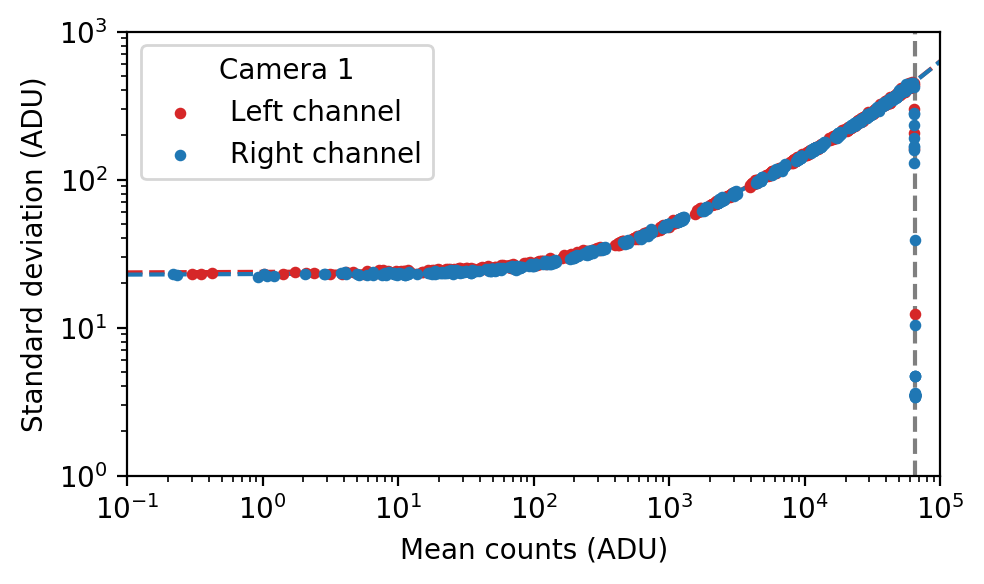
\includegraphics[width=\linewidth]{images/detectors/ptc_1.png}
        \end{minipage}
        \begin{minipage}[t]{0.49\textwidth}\vspace{10pt}
            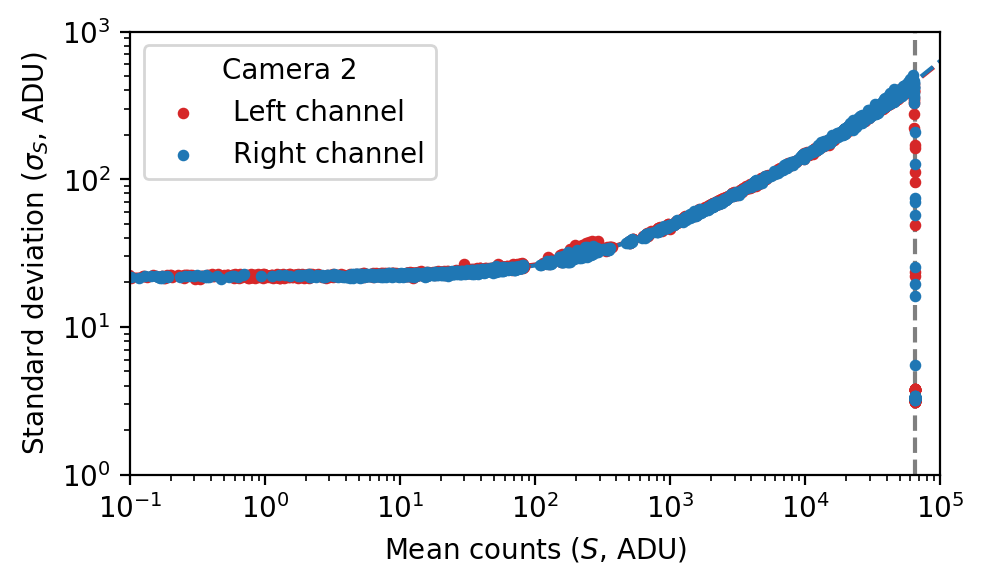
\includegraphics[width=\linewidth]{images/detectors/ptc_2.png}
        \end{minipage}

        \begin{minipage}[t]{0.49\textwidth}\vspace{10pt}
            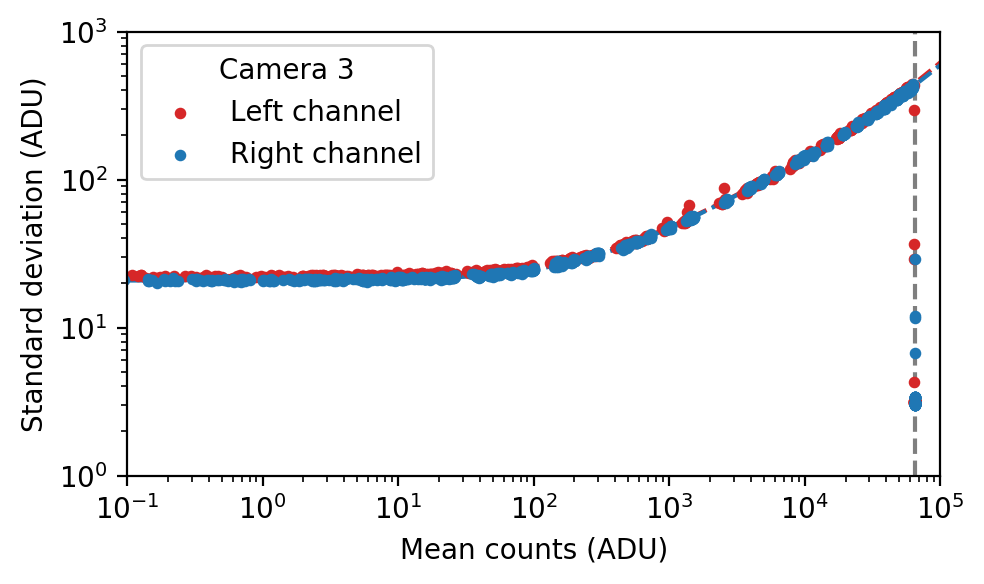
\includegraphics[width=\linewidth]{images/detectors/ptc_3.png}
        \end{minipage}
        \begin{minipage}[t]{0.49\textwidth}\vspace{10pt}
            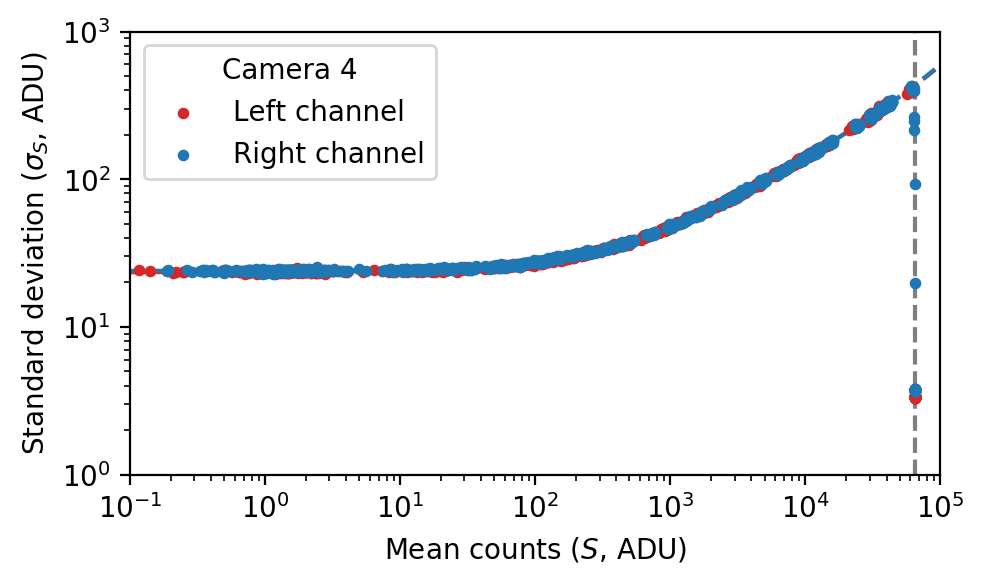
\includegraphics[width=\linewidth]{images/detectors/ptc_4.png}
        \end{minipage}

        \begin{minipage}[t]{0.49\textwidth}\vspace{10pt}
            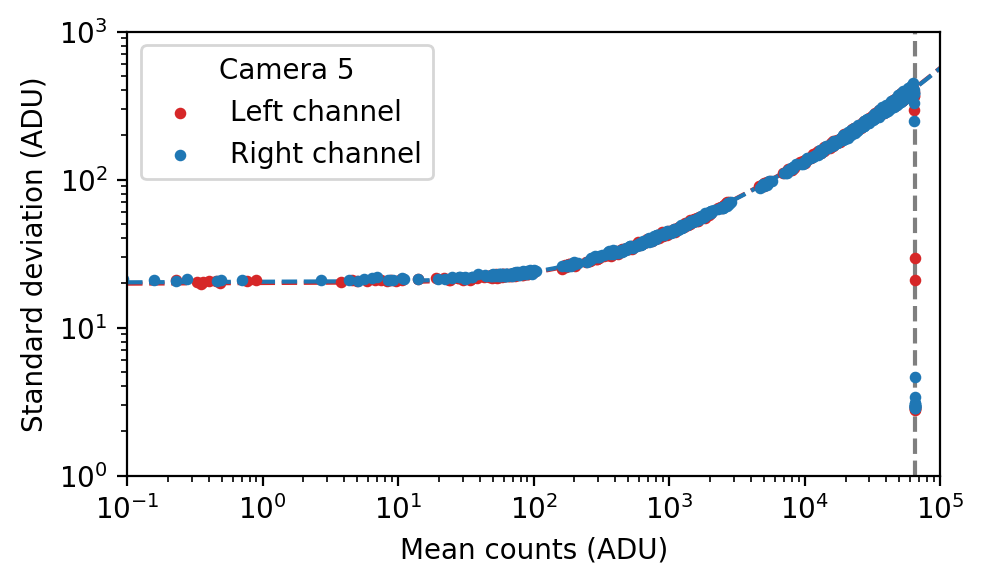
\includegraphics[width=\linewidth]{images/detectors/ptc_5.png}
        \end{minipage}
        \begin{minipage}[t]{0.49\textwidth}\vspace{10pt}
            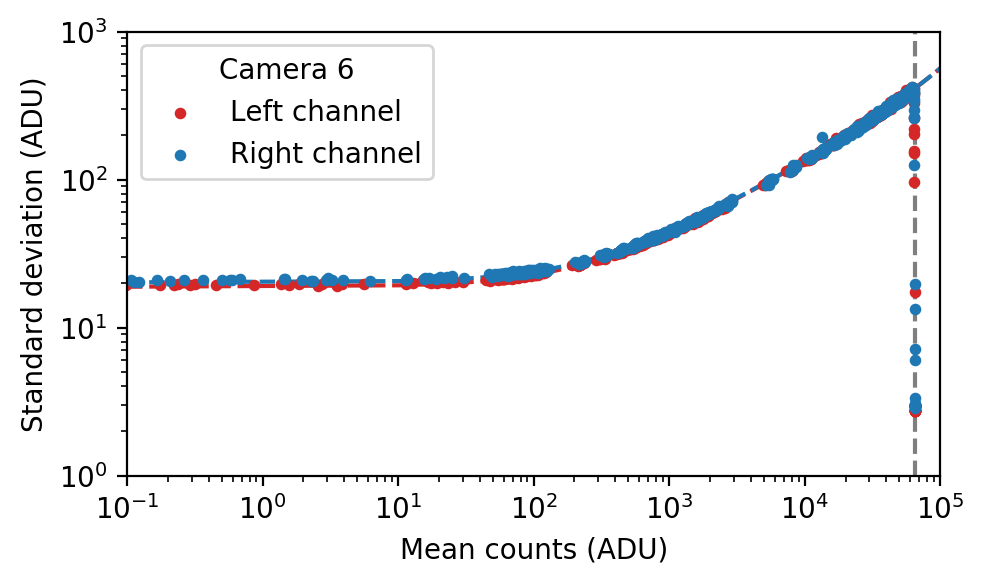
\includegraphics[width=\linewidth]{images/detectors/ptc_6.png}
        \end{minipage}

        \begin{minipage}[t]{0.49\textwidth}\vspace{10pt}
            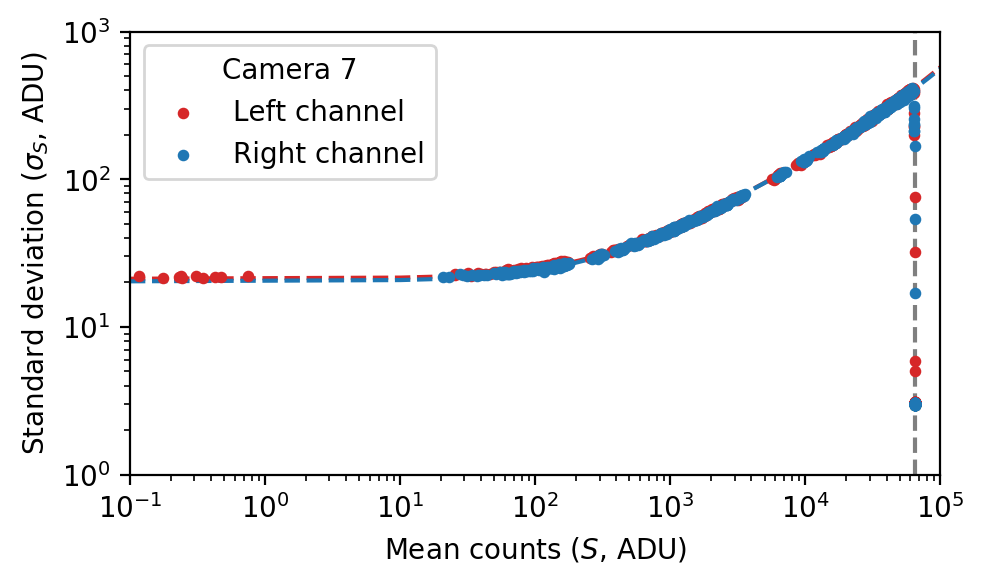
\includegraphics[width=\linewidth]{images/detectors/ptc_7.png}
        \end{minipage}
        \begin{minipage}[t]{0.49\textwidth}\vspace{10pt}
            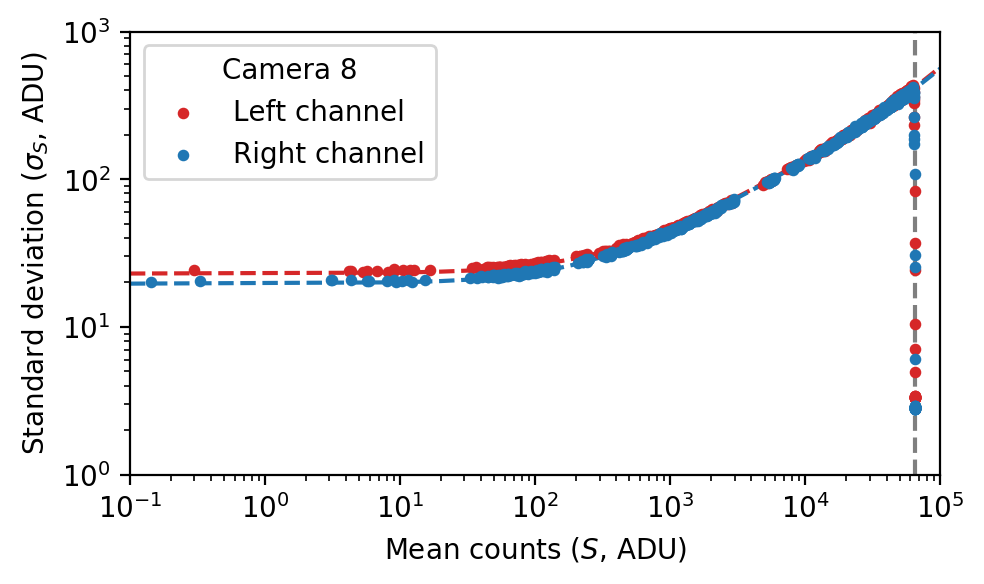
\includegraphics[width=\linewidth]{images/detectors/ptc_8.png}
        \end{minipage}
    \end{center}
    \caption[Photon transfer curves for all 8 cameras]{
        Photon transfer curves for all 8 cameras.
        }\label{fig:ptcs}
\end{figure}

\clearpage

\end{colsection}

% ~~~~~~~~~~~~~~~~~~~~
\newpage
\subsection{Dark current}
\label{sec:dc}
\begin{colsection}

Dark current is another source of noise in a CCD, produced by thermally excited electrons \citep{dark_current}. The dark current noise is therefore independent of the incoming signal or the exposure time, but increases as a function of temperature, $T$. Specifically the dark current increases at an exponential rate and so can be modelled in the form

\begin{equation}
    D(T) = Ae^{kT + C}
    \label{eq:dark_model}
\end{equation}

where $A$, $k$ and $C$ are constants. Dark current is usually defined as doubling after a fixed increase in temperature called the doubling temperature, $T_d$, so that if the dark current $D(T_0) = D_0$ then $D(T_0 + T_d) = 2D_0$. Redefining \aref{eq:dark_model} using these constants gives the equation for dark currant as

\begin{equation}
    D(T) = D_0 e^{\frac{\ln(2)}{T_d}(T + T_0)}.
    \label{eq:dc}
\end{equation}

The choice of $T_0$ is arbitrary, and is usually decided as a reasonable operating temperature by the CCD manufacturer. The FLI specifications give a value for the typical dark current at \SI{-25}{\celsius}, so that is the value of $T_0$ used in this test.

The MicroLine cameras have an in-built fan cooler which can reach \SI{40}{\celsius} below the ambient temperature. In order to find values for the dark current $D_0$ and doubling temperature $T_d$, a series of long (30 minute) dark exposures were taken with each camera at varying temperatures. The mean pixel count was then measured, and divided by 1800 to get the dark current in ADU/second. This value was plotted against temperature as shown in \aref{fig:dcs}. The points were fitted to \aref{eq:dc}, and the resulting values for the dark current and doubling temperature are given in \aref{tab:dc}.

\newpage

\begin{table}[t]
    \begin{center}
        \begin{tabular}{c|cc|cc|rr} %chktex 44
             &
            \multicolumn{4}{c|}{Dark current per pixel} &
            \multicolumn{2}{c}{Doubling} \\
             &
            \multicolumn{4}{c|}{at \SI{-25}{\celsius}} &
            \multicolumn{2}{c}{temperature} \\
             &
            \multicolumn{2}{c|}{(ADU/s)} &
            \multicolumn{2}{c|}{(e-/s)} &
            \multicolumn{2}{c}{(\SI{}{\celsius})} \\
             & L & R & L & R &
             \multicolumn{1}{c}{L} & \multicolumn{1}{c}{R} \\
            \midrule
            Camera 1 & 0.0022 & 0.0017 & 0.0012 & 0.0009 &  7.9 &  6.7 \\
            Camera 2 & 0.0030 & 0.0027 & 0.0016 & 0.0014 &  8.9 &  8.2 \\
            Camera 3 & 0.0034 & 0.0036 & 0.0019 & 0.0020 & 10.7 & 10.9 \\
            Camera 4 & 0.0026 & 0.0030 & 0.0015 & 0.0017 &  9.5 & 10.2 \\
            Camera 5 & 0.0015 & 0.0017 & 0.0009 & 0.0011 &  6.6 &  7.2 \\
            Camera 6 & 0.0020 & 0.0017 & 0.0013 & 0.0011 &  7.5 &  6.8 \\
            Camera 7 & 0.0017 & 0.0014 & 0.0011 & 0.0008 &  7.6 &  6.5 \\
            Camera 8 & 0.0019 & 0.0015 & 0.0012 & 0.0009 &  7.5 &  6.5 \\
        \end{tabular}
    \end{center}
    \caption[TODO]{
        Results of fitting dark current. The conversion from ADU/s to \elec/s used the gain values given in \aref{tab:ptc}.
        }\label{tab:dc}
\end{table}

The FLI MicroLine camera specification for dark current changed between the two test periods; initially it gave a typical per-pixel value of 0.002~\elec/s at \SI{-25}{\celsius}, but in between testing the two sets of cameras that was increased to 0.008~\elec/s. In order to convert the fitted value of dark current in ADU/s to e-/s the individual gain values found from the PTC were used, as listed in \aref{tab:ptc}. All the cameras were found to have a dark current well within the revised specification value, and all except Camera 3 are comfortably below the original 0.002~\elec/s specification.

The KAF-50100 specification includes a value for the dark current doubling temperature of \SI{5.7}{\celsius}, the measured values are all higher: between 6.5--\SI{11}{\celsius}. In practice the temperature dependence of the dark current is not important to GOTO, as the cameras are always cooled to \SI{-25}{\celsius} before images are taken and remain steady at that temperature throughout the night.

The dark current was also examined as a function of time since power on, as in some cameras there are a noticeable amount of free electrons left trapped in the lattice which take time to dissipate \citep{Liam}. No such trend was visible using the FLI cameras. Since the MicroLine cameras have the detector and cooler integrated into the same body there has to be some time spent waiting after power on for the camera to cool to the target temperature before any images could be taken, thus negating the effect.

\begin{figure}[p]
    \begin{center}
        \begin{minipage}[t]{0.49\textwidth}\vspace{10pt}
            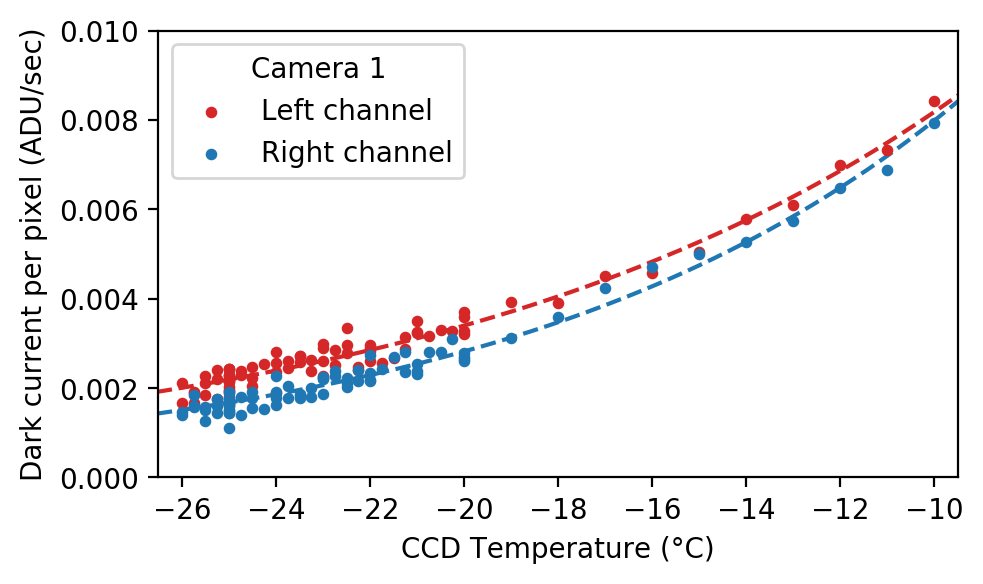
\includegraphics[width=\linewidth]{images/detectors/dc_1.png}
        \end{minipage}
        \begin{minipage}[t]{0.49\textwidth}\vspace{10pt}
            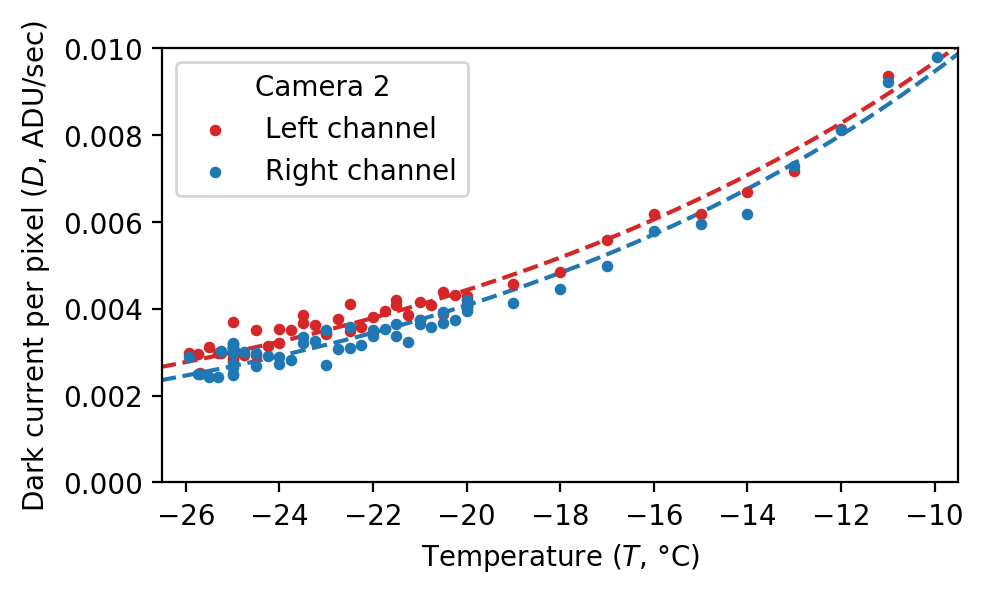
\includegraphics[width=\linewidth]{images/detectors/dc_2.png}
        \end{minipage}

        \begin{minipage}[t]{0.49\textwidth}\vspace{10pt}
            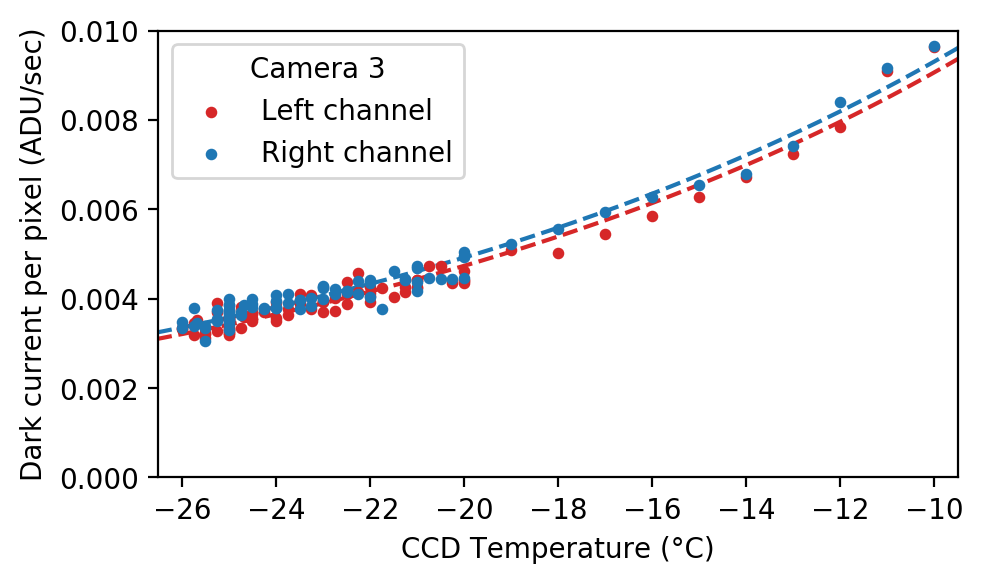
\includegraphics[width=\linewidth]{images/detectors/dc_3.png}
        \end{minipage}
        \begin{minipage}[t]{0.49\textwidth}\vspace{10pt}
            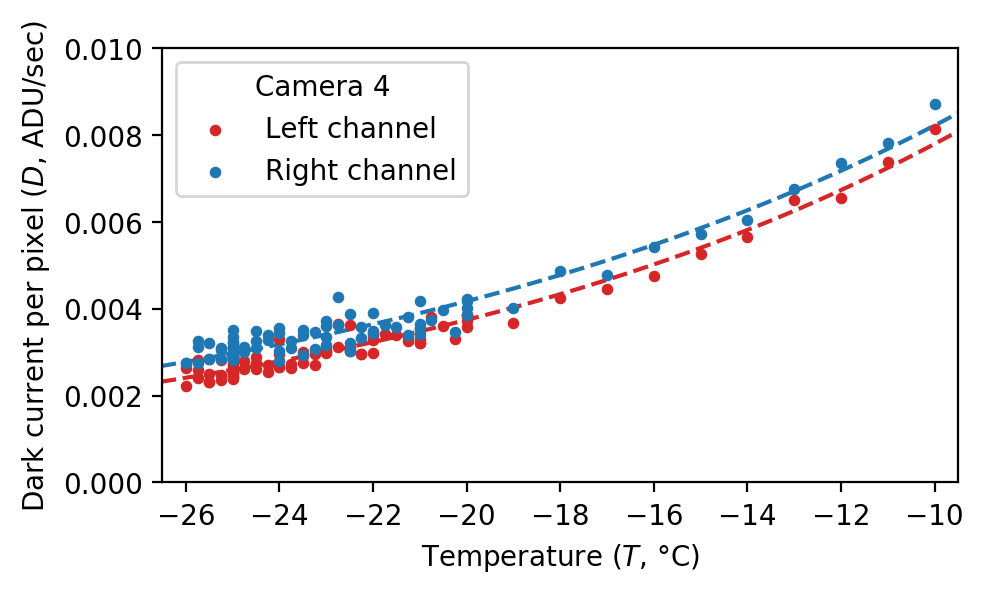
\includegraphics[width=\linewidth]{images/detectors/dc_4.png}
        \end{minipage}

        \begin{minipage}[t]{0.49\textwidth}\vspace{10pt}
            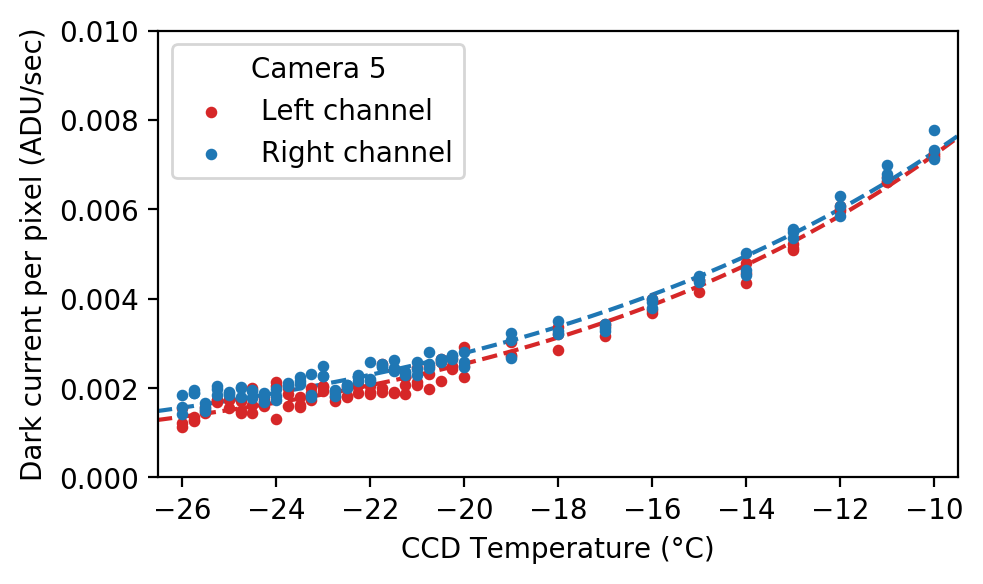
\includegraphics[width=\linewidth]{images/detectors/dc_5.png}
        \end{minipage}
        \begin{minipage}[t]{0.49\textwidth}\vspace{10pt}
            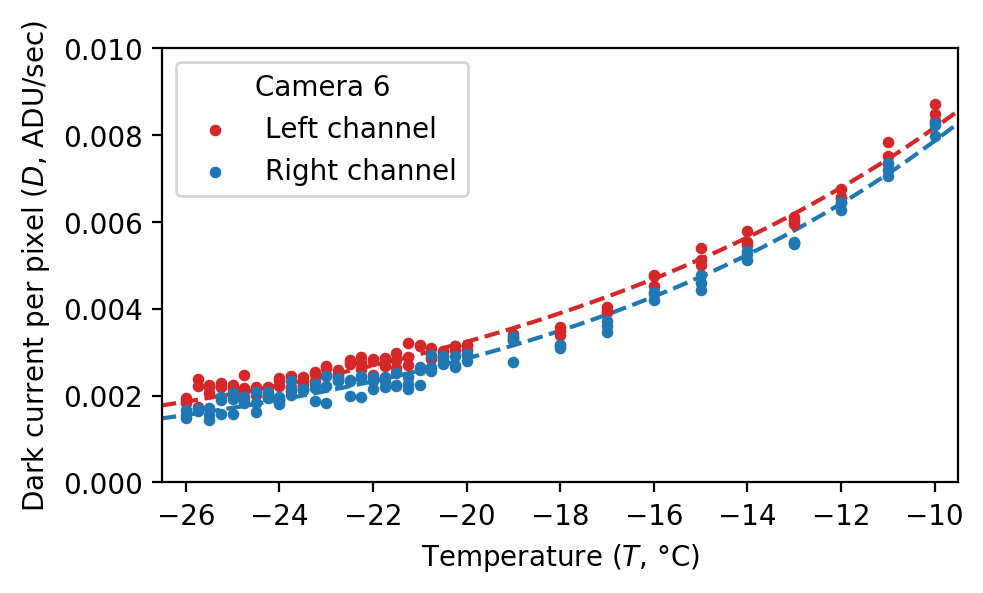
\includegraphics[width=\linewidth]{images/detectors/dc_6.png}
        \end{minipage}

        \begin{minipage}[t]{0.49\textwidth}\vspace{10pt}
            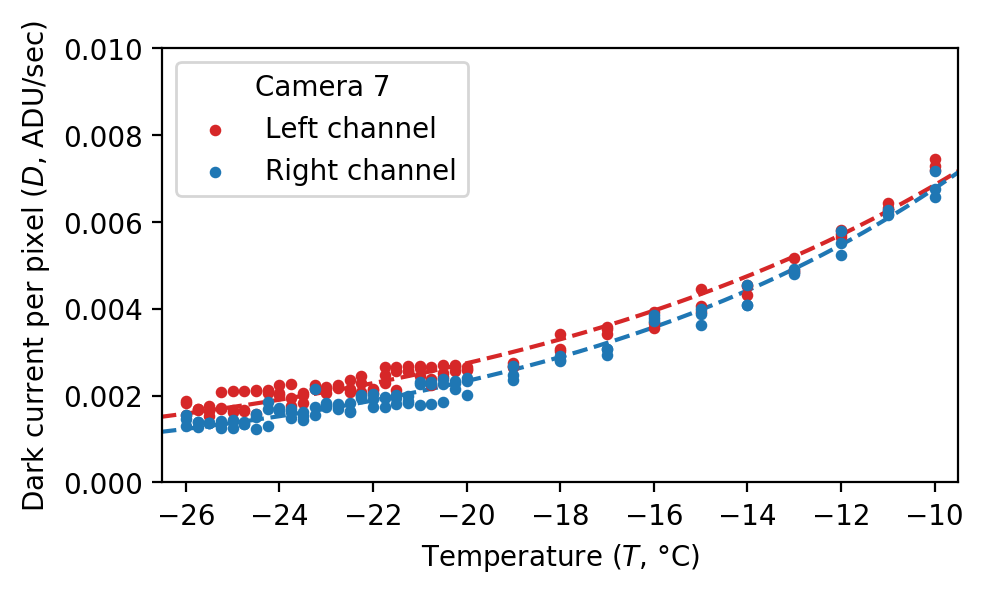
\includegraphics[width=\linewidth]{images/detectors/dc_7.png}
        \end{minipage}
        \begin{minipage}[t]{0.49\textwidth}\vspace{10pt}
            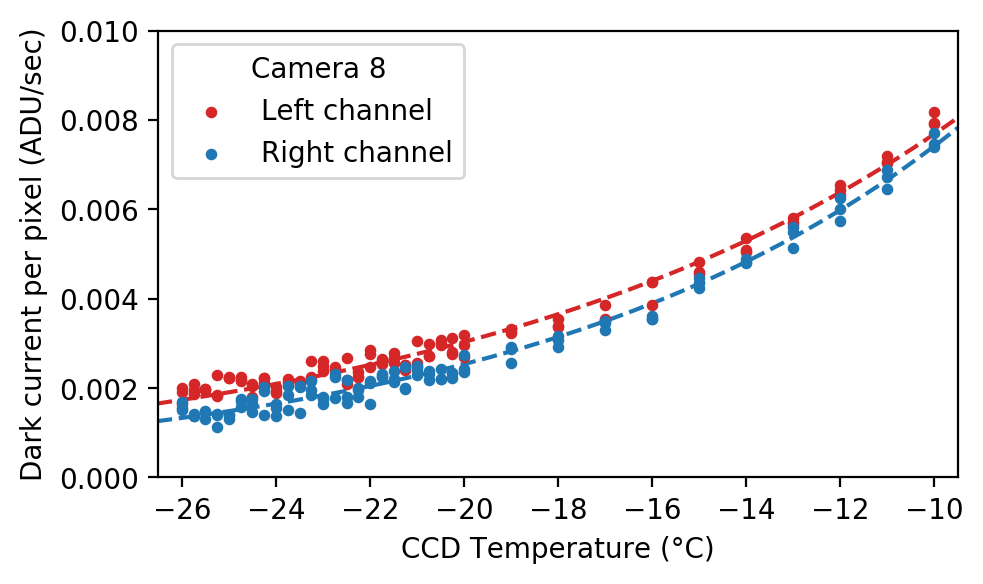
\includegraphics[width=\linewidth]{images/detectors/dc_8.png}
        \end{minipage}
    \end{center}
    \caption[Dark current curves for all 8 cameras]{
        Dark current curves for all 8 cameras.
        }\label{fig:dcs}
\end{figure}

\clearpage

\end{colsection}

% ~~~~~~~~~~~~~~~~~~~~
\newpage
\subsection{Linearity}
\label{sec:linearity}
\begin{colsection}

Linearity was measured for all four cameras using a flat light source and increasing exposure times. Each camera had a turn off in the lower half of the dynamic range which needs further analysis, this experiment was hampered by the broken flat light source. Very short exposure times were studied in order to see any possible effect of the shutter speed. It was found that although the cameras allow exposure times as low as 1ms there is a consistent deviation from linearity below approximately 0.15 seconds. As such exposure times shorter than 0.2 seconds should be avoided.

\end{colsection}

% ~~~~~~~~~~~~~~~~~~~~

\end{colsection}

% ########################################

\newpage
\section{System throughput modelling}
\label{sec:throughput}
\begin{colsection}

% ~~~~~~~~~~~~~~~~~~~~

\begin{colsection}

WIP

\end{colsection}

% ~~~~~~~~~~~~~~~~~~~~
\subsection{Stuff}
\label{sec:stuff}
\begin{colsection}

WIP

\end{colsection}

% ~~~~~~~~~~~~~~~~~~~~

\end{colsection}

% ########################################

\newpage
\section{Deploying the hardware}
\label{sec:hardware}
\begin{colsection}

% ~~~~~~~~~~~~~~~~~~~~

\begin{colsection}

WIP

\end{colsection}

% ~~~~~~~~~~~~~~~~~~~~

\subsection{Construction on La Palma}
\label{sec:construction}
\begin{colsection}

WIP

\end{colsection}

% ~~~~~~~~~~~~~~~~~~~~

\subsection{Extra dome systems}
\label{sec:arduino}
\begin{colsection}

WIP

\end{colsection}

% ~~~~~~~~~~~~~~~~~~~~

\end{colsection}

% ########################################

\newpage
\section{Developing observing routines}
\label{sec:obs_scripts}
\begin{colsection}

% ~~~~~~~~~~~~~~~~~~~~

\begin{colsection}

WIP

\end{colsection}

% ~~~~~~~~~~~~~~~~~~~~

\subsection{Taking flat fields}
\label{sec:flats}
\begin{colsection}

WIP \citep{flats}

\end{colsection}

% ~~~~~~~~~~~~~~~~~~~~

\subsection{Focusing the telescopes}
\label{sec:autofocus}
\begin{colsection}

WIP \citep{autofocus}

\end{colsection}

% ~~~~~~~~~~~~~~~~~~~~

\end{colsection}

% ########################################
